% document formatting
\documentclass[10pt]{article}
\usepackage[utf8]{inputenc}
\usepackage[left=1in,right=1in,top=1in,bottom=1in]{geometry}
\usepackage[T1]{fontenc}
\usepackage{xcolor}

% math symbols, etc.
\usepackage{amsmath, amsfonts, amssymb, amsthm}

% lists
\usepackage{enumerate}

% images
\usepackage{graphicx} % for images

% code blocks
\usepackage{minted, listings} 

% verbatim greek
\usepackage{alphabeta}

\graphicspath{{./assets/images/Week 2}}

\newcommand{\solution}{\textbf{Solution:}} 
\newcommand{\example}{\textbf{Example: }}
\newcommand{\water}{\text{H$_2$O}}
\newcommand{\hydroxide}{\text{OH$^-$}}
\newcommand{\hydronium}{\text{H$_3$O$^+$}}
\newcommand{\proton}{\text{H$^+$}}
\newcommand{\pc}{$^+$}
\newcommand{\nc}{$^-$}
\newcommand{\ka}{\text{$K_\text{a}$}}

\title{CHEM 153A Week 2}

\author{Aidan Jan}
\date{\today}

\begin{document}
\maketitle

\section*{Ionization Constants}
\begin{itemize}
    \item The tendency for any acid (HA) to lose a proton and form its conjugate base (A\nc) is defined by the equilibrium constant (K$_{\text{eq}}$) for the reversible reaction
    \begin{center}
        HA $\rightleftharpoons$ H\pc + A\nc
    \end{center}
    for which 
    \[K_{eq} = \frac{[\text{H}^+][\text{A}^-]}{[\text{HA}]} = K_a\]
\end{itemize}
\subsection*{Acid Strength Comparison: \ka ~and p\ka ~Values of Common Acids}
\begin{center}
    \begin{tabular}{|c|c|c|c|}
        \hline
        No. & \textbf{Acid} & $K_a$ & p$K_a$ \\ \hline
        1 & Hydroiodic acid (HI) & $3.16\times 10^9$ & -9.5 \\ \hline
        2 & Hydrobromic acid (HBr) & $1.0\times 10^9$ & -9 \\ \hline
        3 & Hydrochloric acid (HCl) & $1.0\times 10^6$ & -6 \\ \hline
        4 & Sulfuric acid (H$_2$SO$_4$) & $1.0\times 10^3$ & -3 \\ \hline
        5 & Hydronium ion (\hydronium) & $55$ & -1.74 \\ \hline
        6 & Nitric acid (HNO$_3$) & $28.2$ & -1.45 \\ \hline
        7 & Trifluoroacetic acid (CF$_3$COOH) & $5.62\times 10^{-1}$ & 0.25 \\ \hline
        8 & Oxalic acid (HOOC-COOH) & $5.37\times 10^{-2}$ & 1.27 \\ \hline
        9 & Acetic acid (CH$_3$COOH) & $1.75\times 10^{-5}$ & 4.76 \\ \hline
        \end{tabular}
\end{center}

\subsection*{p\ka}
\begin{itemize}
    \item p\ka = analogous to pH and defined by the equation
    \[p\ka = \log \frac{1}{\ka} = -\log \ka\]
    \item the stronger the tendency to dissociate a proton, the \underline{\textbf{stronger the acid} and \textbf{the lower its p\ka}}
    \item p\ka can be determined experimentally
\end{itemize}
\subsection*{Titration Curves Reveal the p\ka of Weak Acids}
\begin{itemize}
    \item titration curve = a plot of pH against the amount of OH equivalents added
\end{itemize}
\begin{center}
    \includegraphics*[scale=0.8]{L1_1.png}
\end{center}
\subsubsection*{Comparison of the Titration Curves of Three Weak Acids}
\begin{itemize}
    \item a \textbf{weak acid} and its anion - a conjugate acid-base pair - can act as a \textbf{buffer}
    \item Titration curves for acetic acid, dihydrogen phosphate, and ammonium are shown below
    \item \textbf{Conjugate acid-base pairs are effective buffers between approximately 10\% and 90\% neutralization of the proton donor species}
\end{itemize}
\begin{center}
    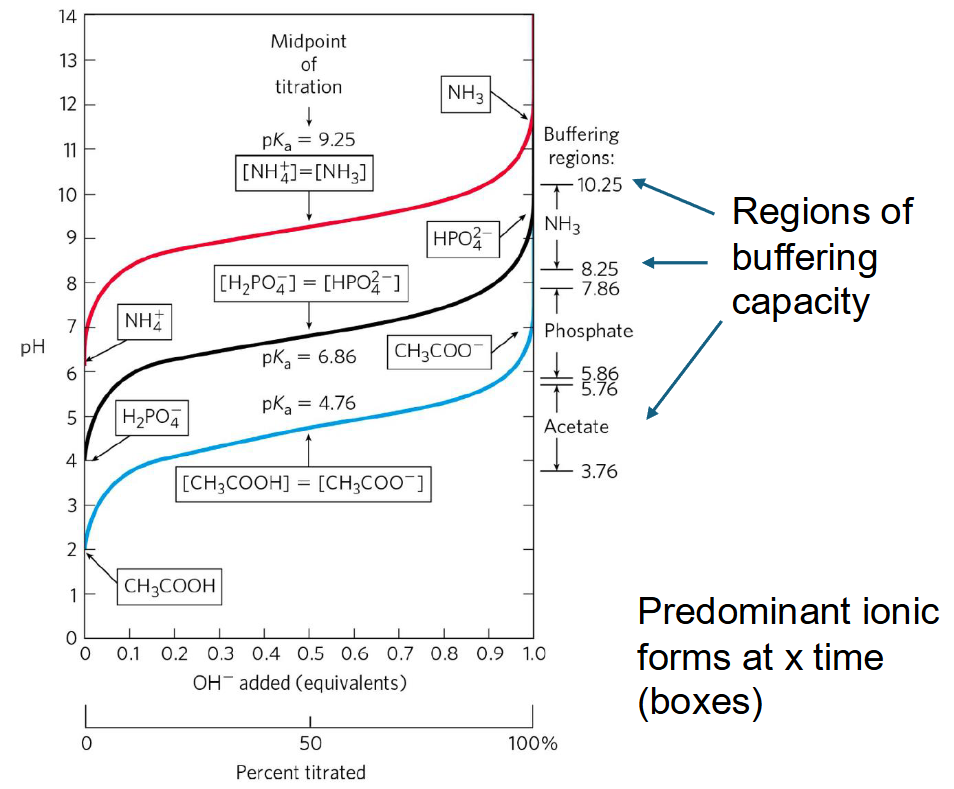
\includegraphics[scale=0.5]{L1_2.png}
\end{center}
\subsection*{Buffers are Mixtures of Weak Acids and Their Conjugate Bases}
\begin{itemize}
    \item buffers = aqueous systems that tend to resist changes in pH when small amounts of acid (\proton) or base (\hydroxide) are added
    \item a buffer system consists of a weak acid (the proton donor) and its conjugate acid (the proton acceptor)
    \item The \textbf{buffering region} is the flat zone of a titration curve (see above)
    \begin{itemize}
        \item the boundaries of a buffer system are pH = p\ka $\pm 1$ (so acetic acid buffer range is 3.76-5.76)
    \end{itemize}
\end{itemize}
\fbox{
    \parbox{\textwidth}{
        The buffering capacity is strongest when the ration of [HA] to [A$^-$] is close to 1:1.  This occurs at the p\ka of the weak acid, where half of the weak acid is dissociated.\\\\
        \textbf{If the ratio of acid to base (or base to acid) becomes too large -} greater than 10:1 or less than 1:10 - the buffer's capacity to neutralize added acids or bases weakens significantly
    }
}
\subsection*{The Henderson-Hasselbalch Equation Relates pH, p\ka, and Buffer Concentration}
\begin{itemize}
    \item \textbf{Henderson-Hasselbalch equation} = describes the shape of the titration curve of any weak acid
    \[\text{pH} = p\ka + \log \frac{[\text{A}^-]}{\text{HA}}\]
    \item Equation only works within the buffer region, outside of this it starts becoming inaccurate
\end{itemize}
\subsubsection*{Primary Uses of the Henderson-Hasselbalch Equation}
\begin{enumerate}
    \item Calculating pH of Buffers
    \begin{itemize}
        \item Predicts pH based on acid/base ratios
    \end{itemize}
    \item Designing Buffers
    \begin{itemize}
        \item Helps create buffers with a desired pH by adjusting the acid-base ratio.
    \end{itemize}
    \item Estimating p\ka
    \begin{itemize}
        \item Can determine the pKa of weak acids and bases experimentally
    \end{itemize}
\end{enumerate}
\subsection*{Deriving the Henderson-Hasselbalch Equation (not needed for exam)}
\begin{align*}
    K_a &= \frac{[\proton][\text{A}^-]}{[\text{HA}]}\\
    [\proton] &= K_a \cdot \frac{[\text{HA}]}{[\text{A}^-]}\\
    -\log [\proton] &= -\log K_a -\log \frac{[\text{HA}]}{[\text{A}^-]}\\
    \text{pH} &= \text{p\ka} -\log \frac{[\text{HA}]}{[\text{A}^-]}\\
    \text{pH} &= \text{p\ka} +\log \frac{[\text{A}^-]}{[\text{HA}]}
\end{align*}
\section*{Amino Acids}
\begin{itemize}
    \item In every living organism, proteins are constructed from a common set of 20 amino acids*
    \item Each amino acid has a side chain with distinctive chemical properties.  Amino acids may be regarded as the alphabet in which the language of protein structure is written.
\end{itemize}
\begin{center}
    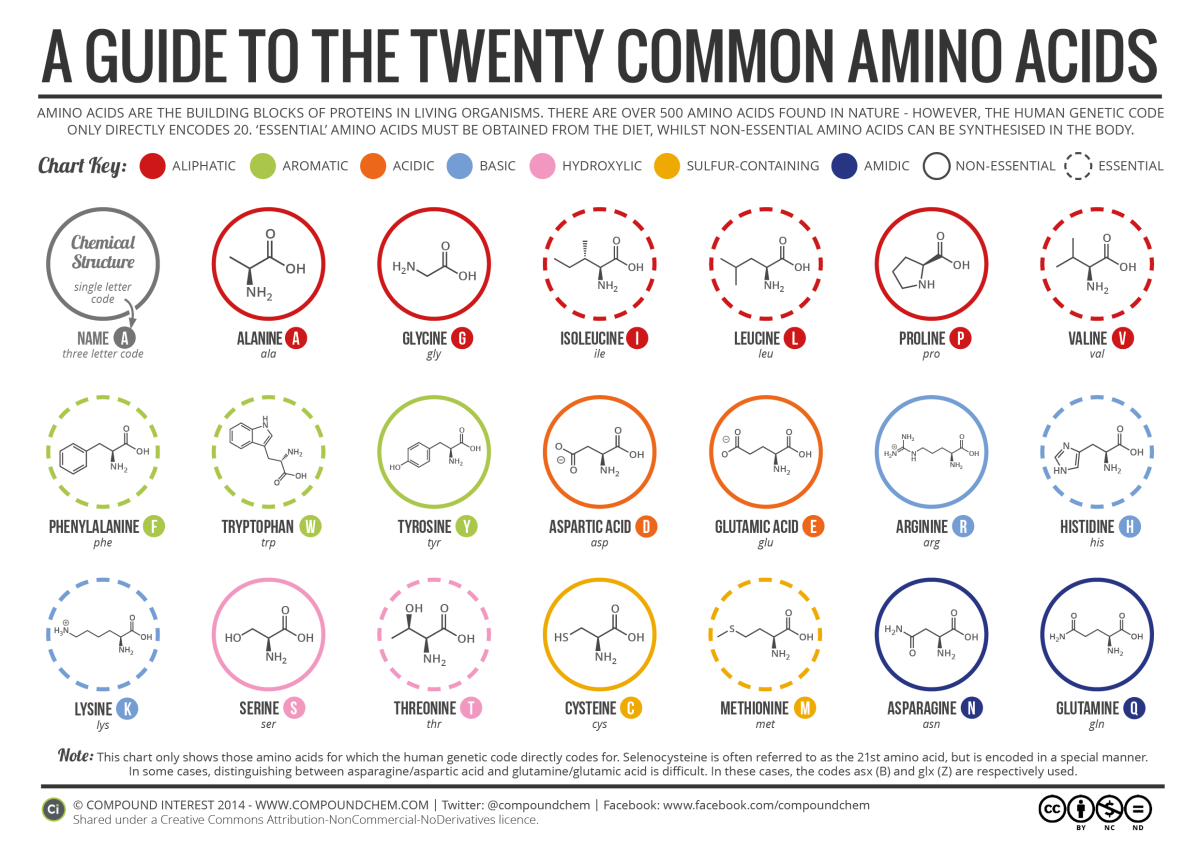
\includegraphics[width=\textwidth]{L1_4.png}
\end{center}
\subsection*{Amino Acids Share Common Structural Features}
\begin{itemize}
    \item $\alpha$ carbon and four substituents
    \item $\alpha$ carbon is the \textbf{chiral center} (except in Glycine, which is not chiral)
    \item Tetrahedral
\end{itemize}
The four substituents are:
\begin{itemize}
    \item a carboxyl group
    \item an amino group
    \item a hydrogen atom
    \item an \textbf{R group} (a side chain unique to each amino acid)
    \begin{itemize}
        \item \textbf{Glycine} has a second hydrogen atom instead of an R group.
    \end{itemize}
\end{itemize}   
\begin{center}
    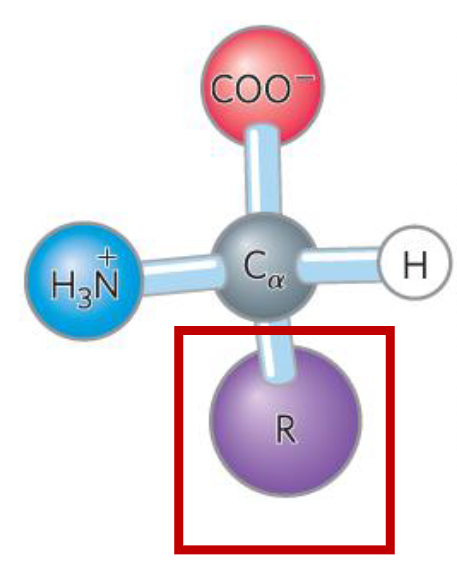
\includegraphics[scale=0.5]{L1_5.png}
\end{center}
\subsection*{The Amino Acid Residues in Proteins are L Stereoisomers}
\begin{itemize}
    \item Two possible stereoisomers = \textbf{enantiomers}
    \item \textbf{optically active} = polarize light is rotated in different directions by enantiomers (Glycine is the exception)
    \item D, L system specifies \textbf{absolute configuration}
\end{itemize}
\begin{center}
    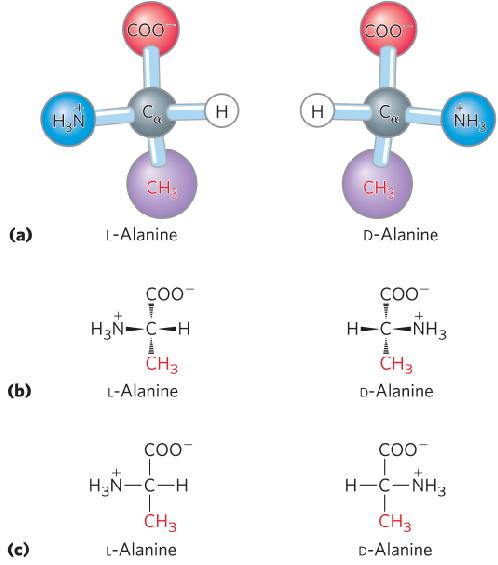
\includegraphics[scale=0.75]{L1_6.png}
\end{center}
\subsection*{Amino Acids can be classified by the R Group}
There are five main classes:
\begin{itemize}
    \item Nonpolar, aliphatic (7)
    \item Aromatic (3)
    \item Polar, uncharged (5)
    \item Positively charged, Basic (3)
    \item Negatively charged, Acidic (2)
\end{itemize}
\subsubsection*{Nonpolar, Aliphatic R Groups}
The \textbf{hydrophobic effect} stabilizes protein structure
\begin{itemize}
    \item Glycine
    \item Alanine
    \item Proline
    \item Valine
    \item Leucine
    \item Isoleucine
    \item Methionine
\end{itemize}

\subsubsection*{Aromatic R Groups}
R groups absorb UV light at 270-280 nm, and can contribute to the hydrophobic effect.
\begin{itemize}
    \item Phenylalanine
    \item Tyrosine
    \item Tryptophan
\end{itemize}

\subsubsection*{Polar, Uncharged R Groups}
R groups can \textbf{form hydrogen bonds}, and Cysteine can \textbf{form disulfide bonds}
\begin{itemize}
    \item Serine
    \item Threonine
    \item Cysteine
    \item Asparagine
    \item Glutamine
\end{itemize}

\subsubsection*{Positively Charged R Groups}
Have significant positive charge at pH 7.0.
\begin{itemize}
    \item Lysine
    \item Arginine
    \item Histidine
\end{itemize}

\subsubsection*{Negatively Charged R Groups}
Have net negative charge at pH 7.0.
\begin{itemize}
    \item Aspartate
    \item Glutamate
\end{itemize}
\subsection*{Essential Amino Acids}
\begin{center}
    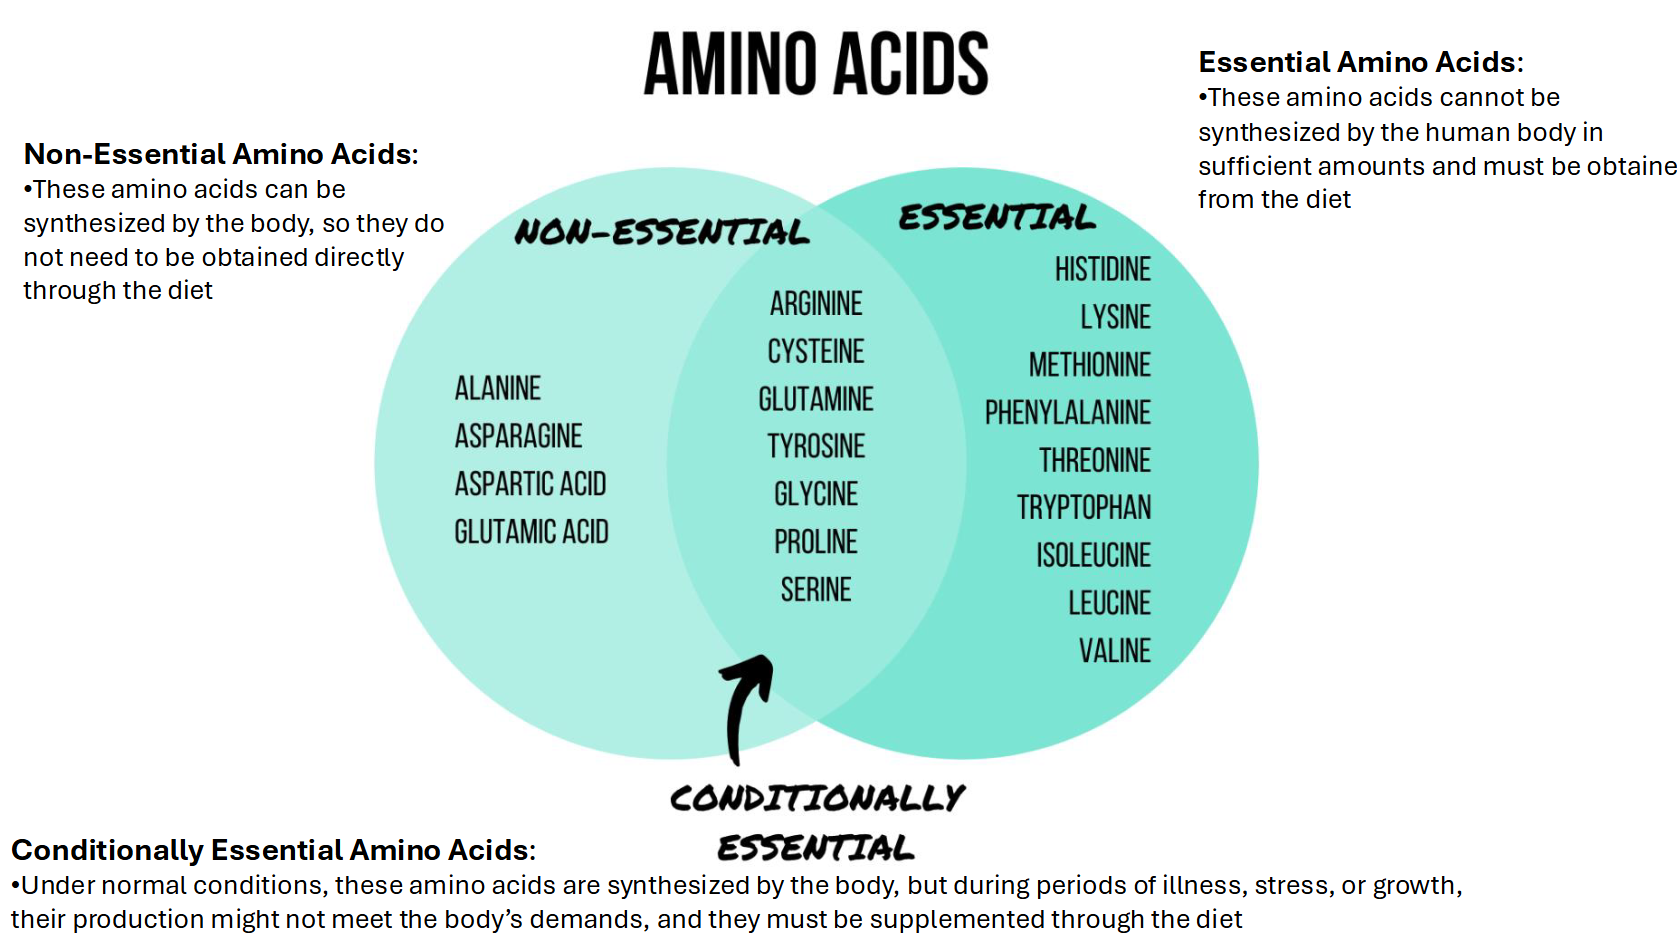
\includegraphics[width=\textwidth]{L1_7.png}
\end{center}
\subsection*{Amino Acids can act as Acids or Bases}
\begin{itemize}
    \item Amino acids are \textbf{acids}.  They are also \textbf{bases} containing an amino group.
    \item The term \textbf{amphoteric} is often used to describe amino acids, meaning that they are capable of acting as both acids and bases
    \item \textbf{zwitterion} occurs at neutral pH.
\end{itemize}
\begin{center}
    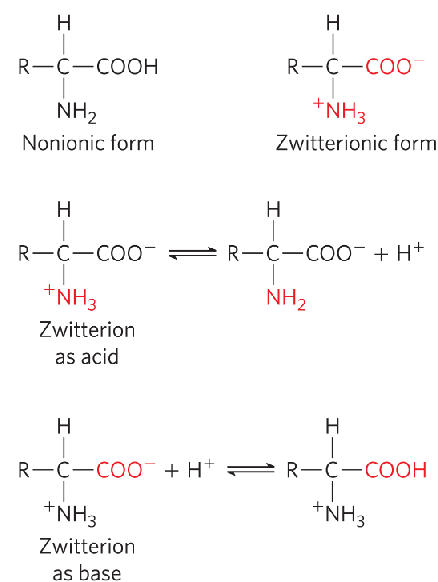
\includegraphics[scale=0.6]{L1_8.png}
\end{center}
\subsubsection*{The pH-dependent structures of a typical amino acid}
For a typical amino acid with a neutral sidechain \textbf{R}:
\begin{itemize}
    \item the positively charged form (+1) dominates at low pH.
    \item the zwitterionic (neutral) form dominates at intermediate pH, and
    \item the negatively charged form (-1) dominates at high pH.
\end{itemize}
\begin{center}
    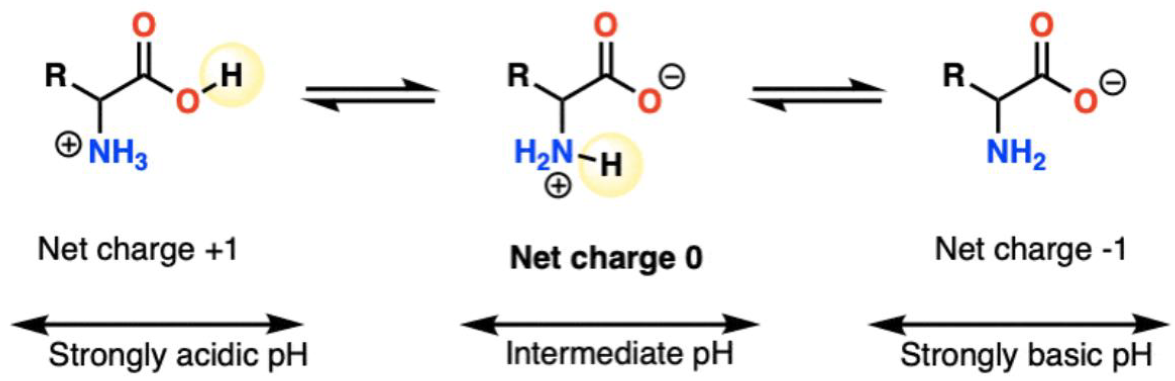
\includegraphics[width=\textwidth]{L1_9.png}
\end{center}
\subsection*{Effect of the Chemical Environment on p\ka}
\begin{itemize}
    \item $\alpha$-carboxyl group is more acidic than in carboxylic acids
    \item $\alpha$-amino group is less basic than in amines
\end{itemize}
\begin{center}
    \includegraphics*[width=\textwidth]{L1_10.png}
\end{center}
\subsection*{Structures (and p\ka) values of selected amino acids}
\begin{center}
    \includegraphics*[width=\textwidth]{L1_11.png}
\end{center}
\end{document}
